\subsection{Raspberry Pi und Qt}
\label{subsec:rasPiUndQt}
Nachde ein grober Überblick zu Qt geschaffen wurde, soll nun eine beispielhafte Anwendung
mithilfe von Qt auf dem Raspberry Pi implementiert werden. Bei dieser Anwendung sollen beim
Betätigen eines Buttons Daten von dem Raspberry Pi gelesen werden und auf der \ac{gui} angezeigt
werden. Dieses Beispiel ist von dem Embedded Systems 2 Labor inspiriert.

\subsubsection{RTIMULib}
\label{subsubsec:RTIMULib}
Die RTIMU Bibliothek war anfändlich dazu gedacht, mithilfe von C++ oder
Python Daten von einem Non-Deeply Embedded System zu lesen. Mitlerweile existiert diese
Bibliothek auch für andere Sprachen wie zum Beispiel C\#.
\newline
\newline
Mithilfe dieser Bibliothek sollen für dieses Beispiel die Daten von dem Raspberry Pi gelesen
werden, um diese dann anschließend auf der \ac{gui} anzeigen zu können. Um RTIMU in einem QT
Projekt nutzen zu können, muss die Bibliothek zunächst in der \emph{.pro} Datei eingebunden
werden. Dies geschieht, indem die Zeile \emph{LIBS += -lRTIMULib} hinzugefügt wird.

\subsubsection{Hilfsklasse}
\label{subsubsec:Hilfsklasse}
Nachdem die Bibliothek hinzugefügt wurde, soll eine Hilfsklasse als Repräsentation der Daten
erzeugt werden. Das folgende Listing zeigt dies auf:

\begin{lstlisting}[language=C++, caption=RTIMU-Hilfsklasse, label=lst:Hilfsklasse]
class ReadData
{
private:
    float m_Temperature = 0.1f;
    float m_AirPressur = 0.1f;
    float m_Humidity = 0.1f;
    float m_xMagnetometer = 0.1f;
    float m_yMagnetometer = 0.1f;
    float m_zMagnetometer = 0.1f;

    RTIMUSettings* m_RTIMUSettings = nullptr;
    RTIMU* m_RTIMU = nullptr;
    RTPressure* m_RTPressure = nullptr;
    RTHumidity* m_RTHumidity = nullptr;

public:
    ReadData();
    void vRead(void);
};

\end{lstlisting}

Die Klasse enthält neben dem im Listing \ref{lst:Hilfsklasse} gezeigten Code noch weitere
Methoden, um auf die privaten \emph{Member Variablen} zuzugreifen. Nun müssen im Konstruktor noch
die Variablen konfiguriert und initialisiert werden, dies geschieht folgendermaßen:

\begin{lstlisting}[language=C++, caption=RTIMU-Hilfsklasse-Konstruktor,
    label=lst:HilfsklasseKonstruktor]
ReadData::ReadData()
{
     // Define variables
     m_RTIMUSettings = new RTIMUSettings("RTIMULib");
     m_RTIMU = RTIMU::createIMU(pRTIMUSettings);
     m_RTPressure = RTPressure::createPressure(pRTIMUSettings);
     m_RTHumidity = RTHumidity::createHumidity(pRTIMUSettings);

     // Init
     pRTIMU->IMUInit();
     pRTIMU->setCompassEnable(true);
     pRTPressure->pressureInit();
     pRTHumidity->humidityInit();
}

\end{lstlisting}

Die letzte Komponente der Hilfsklasse, bildet die \emph{vRead} Methode ab, in der dann
schlussendlich die Daten gelesen werden:

\begin{lstlisting}[language=C++, caption=RTIMU-Hilfsklasse mit der Methode vRead,
    label=lst:vRead]
void ReadData::vRead(void)
{
    if (m_RTIMU->IMURead())
    {
        RTIMU_DATA RTIMUData = m_RTIMU->getIMUData();
        m_RTPressure->pressureRead(RTIMUData);
        m_RTHumidity->humidityRead(RTIMUData);

        m_AirPressur = RTIMUData.pressure;
        m_Temperature = RTIMUData.temperature;
        m_fHumidity = RTIMUData.humidity;

        RTIMUData.compass.normalize();
        m_xMagnetometer = RTIMUData.compass.x();
        m_yMagnetometer = RTIMUData.compass.y();
        m_zMagnetometer = RTIMUData.compass.z();
    }
}

\end{lstlisting}

\subsubsection{Benutzeroberfläche}
\label{subsubsec:QtGui}
Die Benutzeroberfläche in diesem Beispiel wurde schlicht gehalten. Sie besitzt insgesamt zwölf
QtLabels wovon sechs dafür gedacht sind, um die Raspberry Pi Daten abzubilden und einem Button,
der die Daten abrufen soll.
\newline
\newline
Der Button wurde mit einem Slot versehen der aufgerufen wird, wenn der Button betätigt wird. In
dem Slot wird die vRead Methode aufgerufen, um dann die Labels zu aktualisieren. Die
Implementierung des Slots sieht dann folgend aus:

\begin{lstlisting}[language=C++, caption=Slot Methode für den Update-Button,
    label=lst:updateSlot]
void MainWindow::on_pbUpdate_clicked()
{
    m_readData->vRead();

    double dValue = static_cast<double>(m_readData->getAirPressur());
    ui->lblLuftdruck->setText(QString::number(dValue));

    dValue = static_cast<double>(m_readData->getTemperature());
    ui->lblTemperatur->setText(QString::number(dValue));

    dValue = static_cast<double>(m_readData->getHumidity());
    ui->lblLuftfreutigkeit->setText(QString::number(dValue));

    dValue = static_cast<double>(m_readData->getMagnetometerX());
    ui->lblKompassX->setText(QString::number(dValue));

    dValue = static_cast<double>(m_readData->getMagnetometerY());
    ui->lblKompassY->setText(QString::number(dValue));

    dValue = static_cast<double>(m_readData->getMagnetometerZ());
    ui->lblKompassZ->setText(QString::number(dValue));
}

\end{lstlisting}

Das vollständige Programm ist in der folgenden Abbildung dargestellt

\begin{figure}[h]
    \centering
    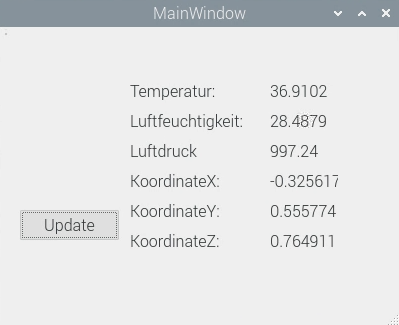
\includegraphics[width=0.55\textwidth, center]{StandDerTechnik/QtGUI}
    \caption[GUI der beispielhaften Anwendung]{GUI der beispielhaften Anwendung}
    \label{img:qtGui}
\end{figure}
